%\documentclass[aspectratio=169]
\documentclass[aspectratio=169,xcolor=dvipsnames]{beamer}
%\usetheme{Copenhagen}
\usetheme{Madrid}
\setbeamertemplate{navigation symbols}{}
%\setbeamertemplate{footline}{}
\usecolortheme[named=Green]{structure}

\usepackage[utf8]{inputenc}

\usepackage{graphicx}         
\graphicspath{ {./Pictures/} }
\usepackage{amsmath}
\usepackage{amsfonts}
\usepackage{amssymb}
\usepackage{amsthm}
\usepackage{mathtools}
\usepackage{commath}
\usepackage{multimedia}
\usepackage{subcaption}
\usepackage{media9}
\addmediapath{Animations/}
\newcommand{\Sta}{y}
\newcommand{\Adj}{p}
\newcommand{\Con}{u}
\begin{document}

\title[]{This Is What We Do: \\
PDE-Constrained Optimization for Multiscale Particle Dynamics}
\author[Jonna Roden]{Jonna Roden}
\institute[]{With Dr Ben Goddard (UoE), Dr John Pearson (UoE) \\ and Mildred Aduamoah (MIGSAA, 3rd Year)}
\titlepage
 
 
\begin{frame}
	\frametitle{Structure of the Talk}
	 
	 \begin{itemize}
	 	\item Part 1: What is Multiscale Particle Dynamics?
	 	\item Part 2: What is PDE-Constrained Optimization?
	 	\item Part 3: This Is What We Do (Modelling, Numerics, Analysis)
	 \end{itemize}
\end{frame}
\begin{frame}
	\frametitle{Part 1: What is Multiscale Particle Dynamics?}
	
	\begin{columns}
		\column{0.7 \linewidth}	
		What do these pictures have in common?\\
		
		\begin{columns}	
			\column{0.5 \linewidth}
			\begin{figure}
				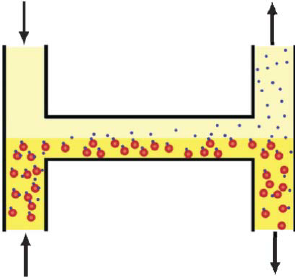
\includegraphics[width=4cm]{Microfilter.png}
				\caption{ Nanofiltration Device}
			\end{figure}
			\column{0.5 \linewidth}
			\begin{figure}		
				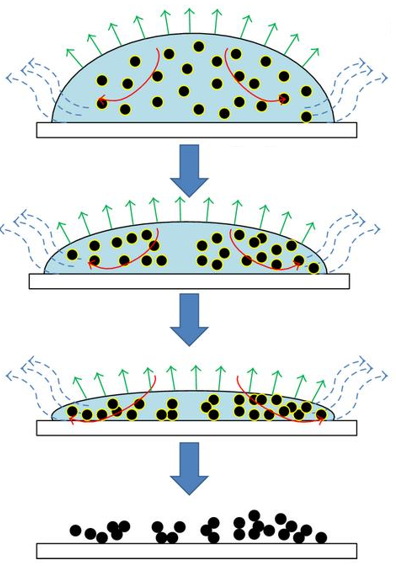
\includegraphics[width=4cm]{printing1.png}
				\caption{Ink Droplet Drying Process}
			\end{figure}
		\end{columns}
		\column{0.3 \linewidth}
		
		\begin{figure}
			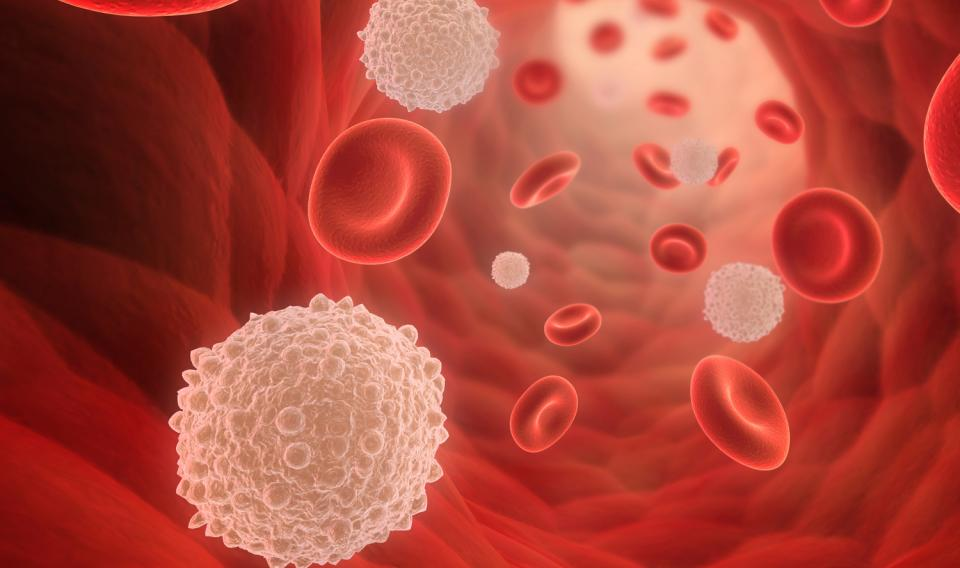
\includegraphics[width=3cm]{bloodcells.jpg}
			\caption{Blood Cells in Blood Vessles}
		\end{figure}
		\begin{figure}
			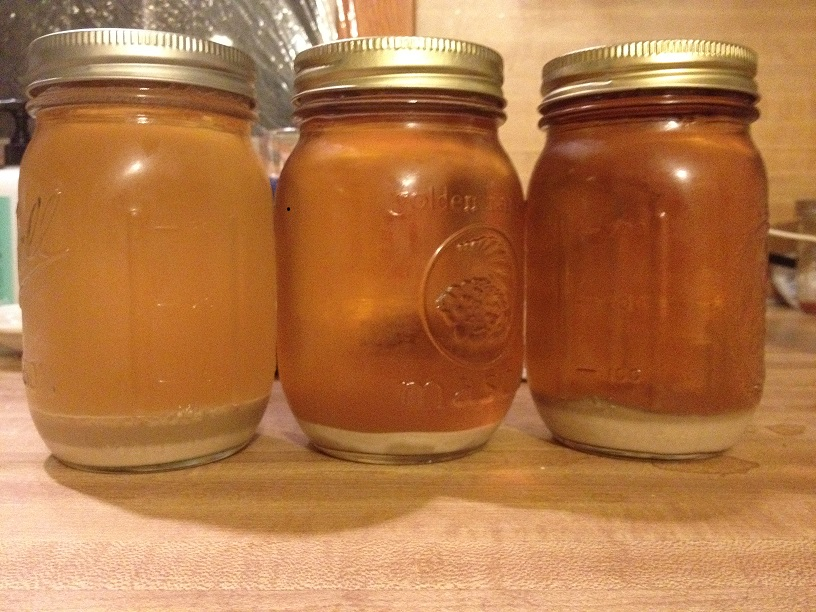
\includegraphics[width=3cm]{beer.jpg}
			\caption{Yeast Sedimentation in Beer}
		\end{figure}
		
	\end{columns}
\end{frame}

\begin{frame}
	\frametitle{Part 1: What is Multiscale Particle Dynamics?}
	 Mathematically, they are like this picture!
	
	\begin{figure}
		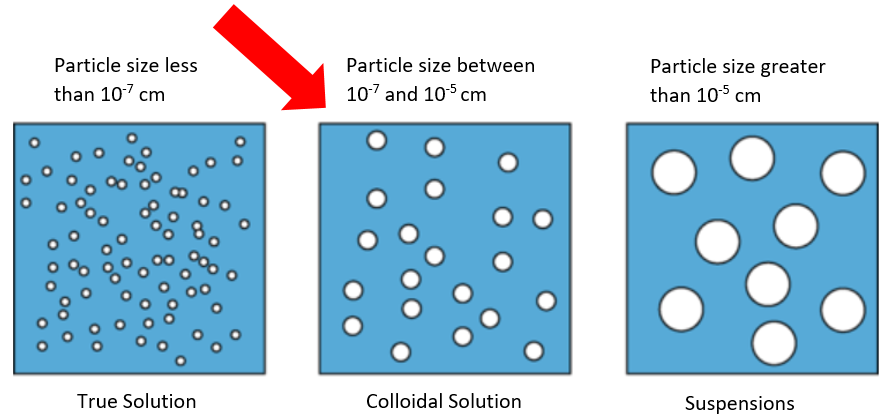
\includegraphics[width=10cm]{Particles2.png}
	\end{figure}
\end{frame}
\begin{frame}
	\frametitle{Part 1: What is Multiscale Particle Dynamics?}
	
	\begin{figure}
		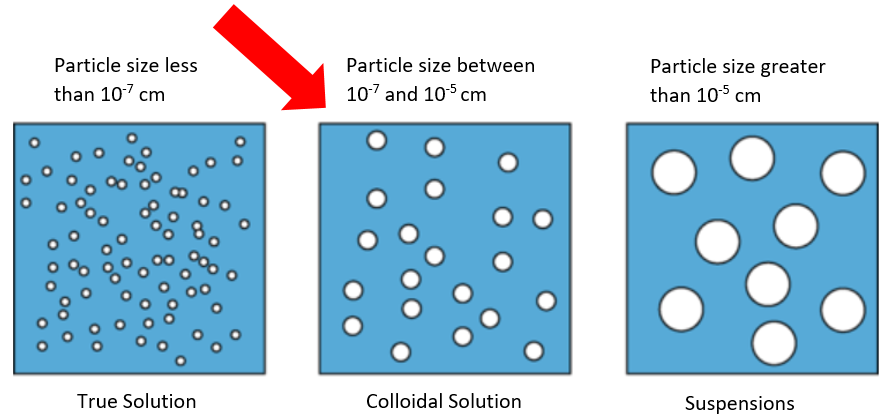
\includegraphics[width=8cm]{Particles2.png}\\
		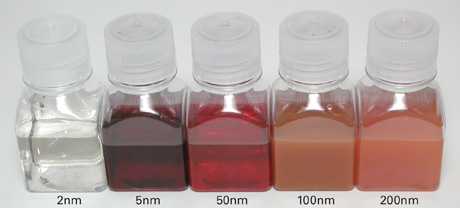
\includegraphics[width=8cm]{GoldColloids.jpg}
	\end{figure}
\end{frame}
\begin{frame}
	\frametitle{Part 1: What is Multiscale Particle Dynamics?}
	How can we describe this picture mathematically?
	\vspace{1cm}
	\begin{columns}
		\column{0.4 \linewidth}

	\begin{figure}
		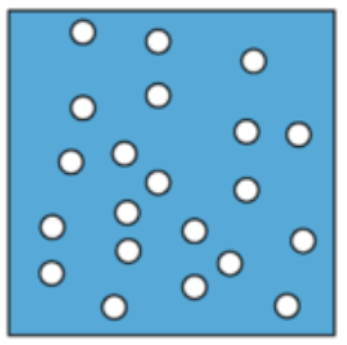
\includegraphics[width=4cm]{Particles3.png}
	\end{figure}
		\column{0.6 \linewidth}
		On Multiple Scales:
		\begin{itemize}
			\item Experimentally 
			\item ODEs for N particles AND n water molecule
			\item SDEs for N particles
			\item PDEs for the N particle density 
			\item PDEs for the 1 particle density 
			\item PDEs for the bulk fluid
		\end{itemize}
	\end{columns}
\end{frame}
\begin{frame}
	\frametitle{Part 1: What is Multiscale Particle Dynamics?}
	How can we describe this picture mathematically?\\
	\vspace{1cm}
	\begin{columns}
		\column{0.3 \linewidth}
		
		\begin{figure}
			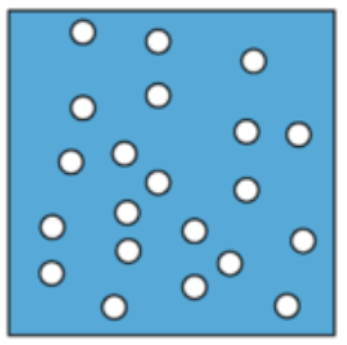
\includegraphics[width=4cm]{Particles3.png}
		\end{figure}
		\column{0.7 \linewidth}
	      On Multiple Scales:
		\begin{itemize}
			\item Experimentally \textcolor{red}{(expensive in cost and time!)}
			\item ODEs for N particles AND n water molecule\\ \textcolor{red}{(impossible computations!)}
			\item SDEs for N particles \textcolor{red}{(expensive computations!)}
			\item PDEs for the N particle density  \textcolor{red}{(expensive computations!)}
			\item PDEs for the 1 particle density \textcolor{green}{(good compromise)}
			\item PDEs for the bulk fluid \textcolor{red}{(inaccurate for many processes!)}
		\end{itemize}
	\end{columns}
\end{frame}

\begin{frame}
	\frametitle{Part 1: What is Multiscale Particle Dynamics?}
Why do we want to describe this mathematically?

	
	\begin{figure}
		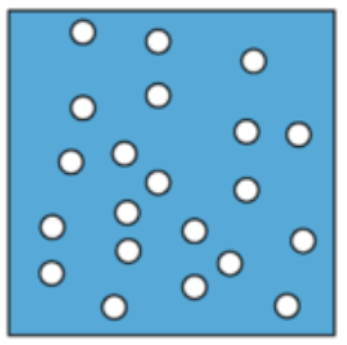
\includegraphics[width=4cm]{Particles3.png}
	\end{figure}

Many processes can be described by this type of fluid model!...
\end{frame}

\begin{frame}
	\frametitle{Part 1: What is Multiscale Particle Dynamics?}
	
	\begin{columns}
		\column{0.7 \linewidth}	
		....Such as these ones!\\
		
		\begin{columns}	
			\column{0.5 \linewidth}
			\begin{figure}
				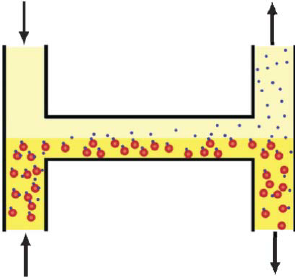
\includegraphics[width=4cm]{Microfilter.png}
				\caption{ Nanofiltration Device}
			\end{figure}
			\column{0.5 \linewidth}
			\begin{figure}		
				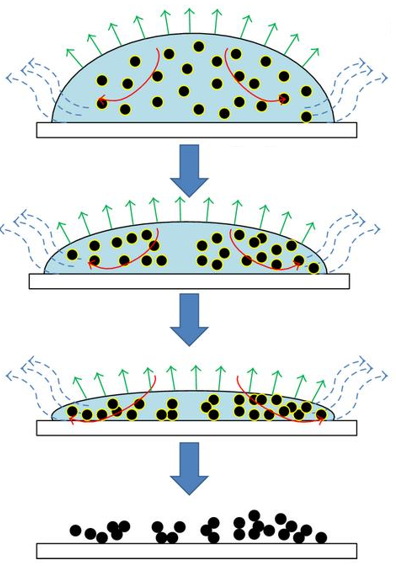
\includegraphics[width=4cm]{printing1.png}
				\caption{Ink Droplet Drying Process}
			\end{figure}
		\end{columns}
		\column{0.3 \linewidth}
		
		\begin{figure}
			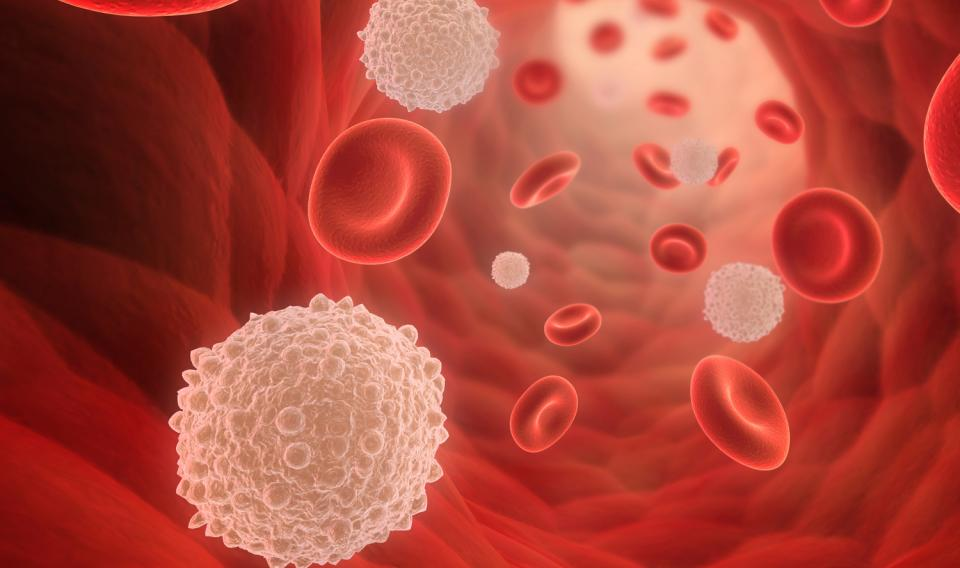
\includegraphics[width=3cm]{bloodcells.jpg}
			\caption{Blood Cells in Blood Vessles}
		\end{figure}
		\begin{figure}
			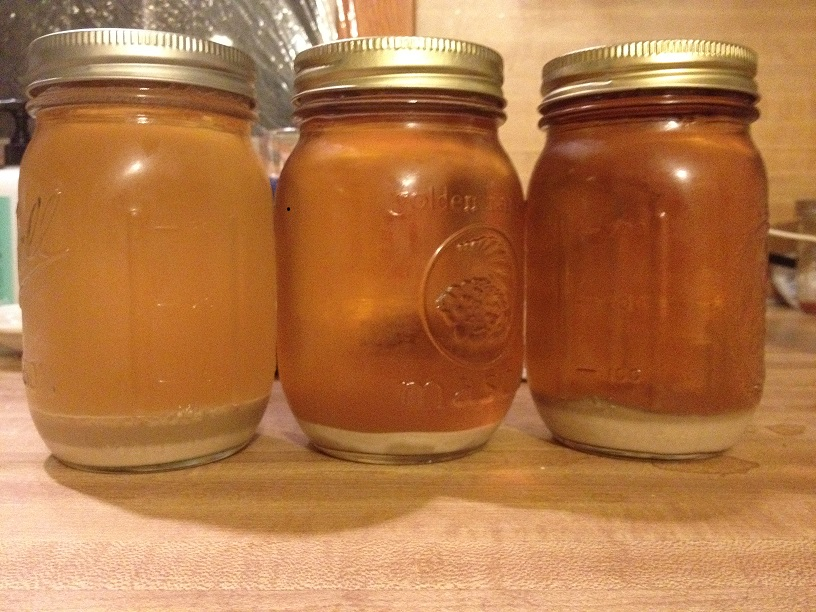
\includegraphics[width=3cm]{beer.jpg}
			\caption{Yeast Sedimentation in Beer}
		\end{figure}
		
	\end{columns}
\end{frame}



\begin{frame}
	\frametitle{Part 1: What is Multiscale Particle Dynamics?}
	
	\begin{columns}
		\column{0.5 \linewidth}
			Two industrial partners of the PhD:
		\begin{figure}
			
\includegraphics[width=4cm]{ufraction8.png}
			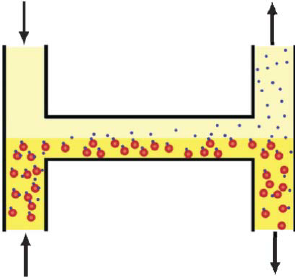
\includegraphics[width=4cm]{Microfilter.png}
			\caption{Nanofiltration Device}
		\end{figure}

		\column{0.5 \linewidth}
		\begin{figure}
			
\includegraphics[width=3.5cm]{west.png}\\
			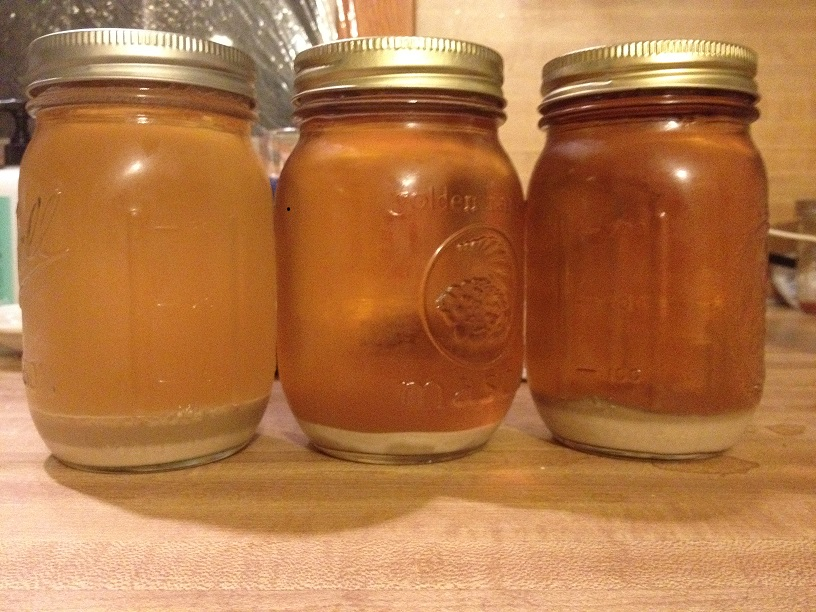
\includegraphics[width=3.5cm]{beer.jpg}
			\caption{Yeast Sedimentation in Beer}
		\end{figure}
	\end{columns}
\end{frame}
\begin{frame}
\frametitle{Part 2: What is PDE-Constrained Optimization? }
\begin{columns}
\column{0.5 \linewidth}
\begin{align*}
&\min_{\rho,u} \quad \frac{1}{2}\norm{\rho- \hat{\rho}}_{L_2}^2 + \frac{\beta}{2} \norm{u}_{L_2}^2,\\
\\
&\text{subject to:}
\\
& \frac{\partial \rho}{\partial t}= \Delta \rho + u 
\end{align*}
\column{0.5 \linewidth}
Example:
\begin{itemize}
	\item $\rho$: Current temperature.
	\item $\hat \rho$: Desired temperature.
	\item $u$: Cost of reaching $\hat \rho$.
	\item PDE: Heat equation.
\end{itemize}
	
\end{columns}
\end{frame}
\begin{frame}
	\frametitle{Part 2: What is PDE-Constrained Optimization? }
	\begin{columns}
		\column{0.3 \linewidth}
		\begin{figure}
			
\includegraphics[width=4cm]{ufraction8.png}
			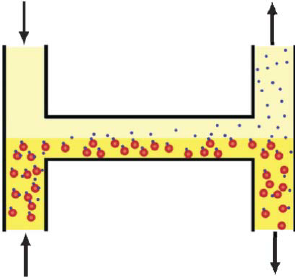
\includegraphics[width=4cm]{Microfilter.png}
			\caption{Nanofiltration Device}
		\end{figure}
		\column{0.4 \linewidth}
		\begin{align*}
		&\min_{\rho,u} \quad \frac{1}{2}\norm{\rho- \hat{\rho}}_{L_2}^2 + \frac{\beta}{2} \norm{u}_{L_2}^2,\\
		\\
		&\text{subject to:}
		\\
		& \frac{\partial \rho}{\partial t}= \Delta \rho + u 
		\end{align*}
		\column{0.3 \linewidth}
		\begin{figure}
		 
\includegraphics[width=3cm]{west.png}\\
		 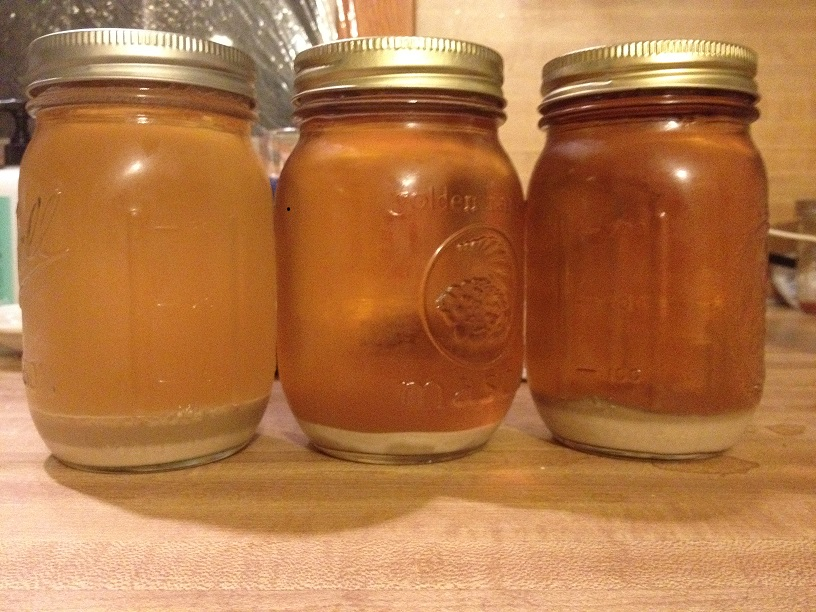
\includegraphics[width=3cm]{beer.jpg}
		 \caption{Yeast Sedimentation in Beer}
		\end{figure}
	
	\end{columns}
\end{frame}

\begin{frame}
	\frametitle{Part 3: What is it that we do?}
	
	\begin{itemize}
		\item Modelling
		\item Numerics
		\item (Analysis)
	\end{itemize}
	
\end{frame}
\begin{frame}
	\frametitle{Part 3: What is it that we do?}
	\begin{columns}
		\column{0.6 \linewidth}
	\textbf{Modelling}: What can we describe with our PDEs?
	\begin{itemize}
		\item Forces
		\item Particle Interactions
		\item Multiple Species
		\item Self-propelled particles
		\item Different Geometries
		\item ...
	\end{itemize}
       \column{0.4 \linewidth}
       		\begin{figure}
       	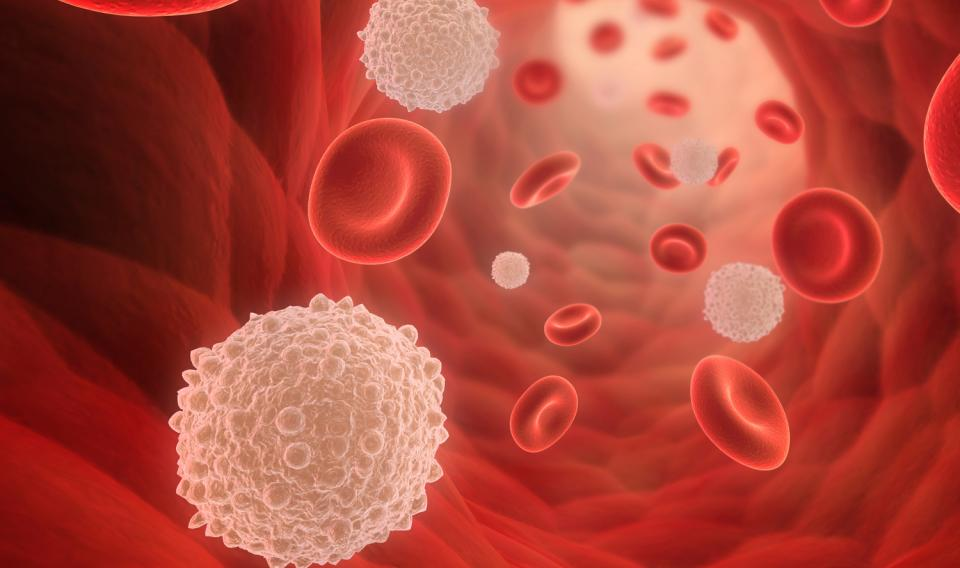
\includegraphics[width=3cm]{bloodcells.jpg}\\
       	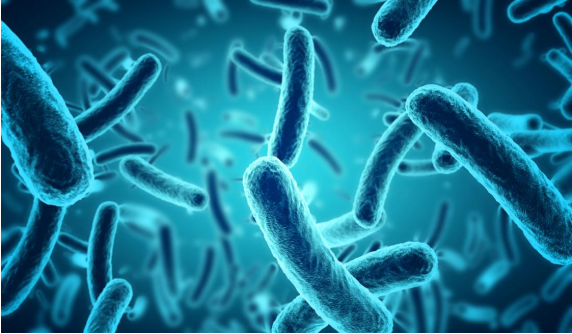
\includegraphics[width=3cm]{bacteria.png}\\
       	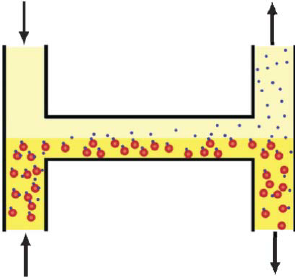
\includegraphics[width=3cm]{Microfilter.png}
       \end{figure}
    \end{columns}
\end{frame}
\begin{frame}
	\frametitle{Part 3: What is it that we do?}

		\textbf{Modelling}: How do we approach the modelling process?
\begin{itemize}
	\item Choose the most basic (but meaningful) model.
	\item Add on \textcolor{red}{one effect}.
	\item Develop numerics for this model (next slide!).
	\item Add on \textcolor{blue}{more effects}, step by step.
	\item Get final model.
\end{itemize}
\begin{align*}
\frac{\partial \rho}{\partial t}= \Delta \rho + \textcolor{red}{u} +\textcolor{blue}{\alpha \int_\Omega \rho(x) \rho(x') \nabla V_2(|x-x'|)dx'}
\end{align*}
\end{frame}
\begin{frame}
	\frametitle{Part 3: What is it that we do?}
\textbf{Numerics}: Optimization = Solving systems of PDEs
	\begin{itemize} 
		\item Challenge: Particle interaction term is nonlinear and non-local.
		\item Standard methods (FEM/FDM) are not enough.
	\end{itemize}
We use:
\begin{itemize}
		\item Pseudospectral methods.
		\item Multiple shooting method.
	\end{itemize}
\end{frame}

\begin{frame}
	\frametitle{Part 3: What is it that we do?}
\textbf{Numerics}: What are pseudospectral methods?\\
\begin{itemize}
	\item Polynomial interpolation using Chebyshev points.
	\item Discretize space: $\Delta \rho \to D \rho$ (PDE $\to$ ODE)
\end{itemize}
 
 
	\begin{figure}
	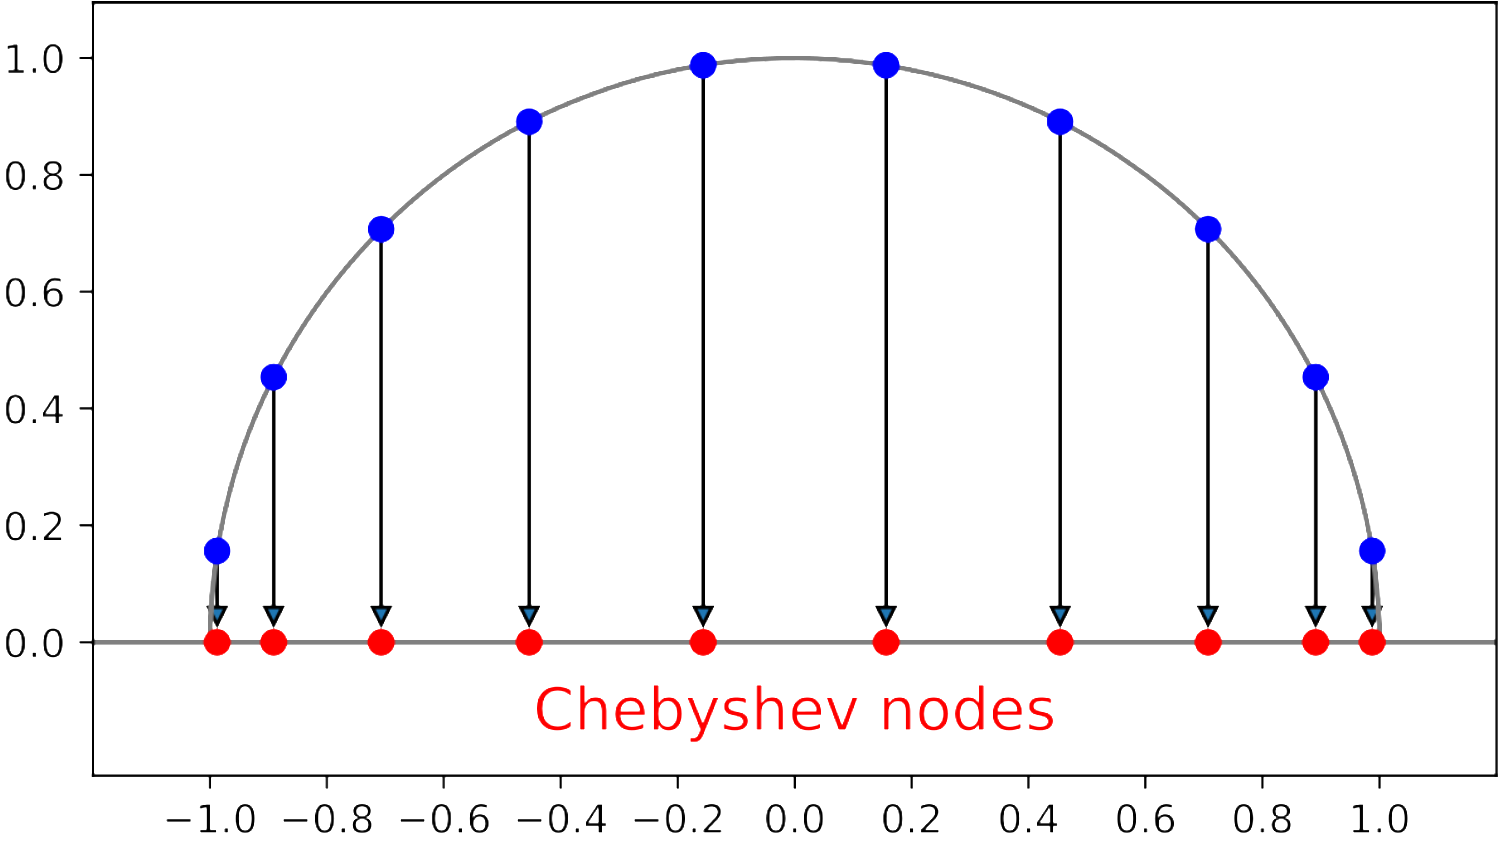
\includegraphics[width=8cm]{chebnodes1.png}\\
	\caption{Chebyshev Points}
\end{figure}	
\end{frame}

\begin{frame}
	\frametitle{Part 3: What is it that we do?}
	\textbf{Numerics}: What is the multiple shooting method?\\
    \begin{itemize}
    	\item Reduce PDEs to ODEs using pseudospectral methods.
    	\item Discretize the time interval, guess solution on $t_i$.
        \item Solve ODEs on each time interval, match endpoints.
    \end{itemize}
	\begin{figure}
		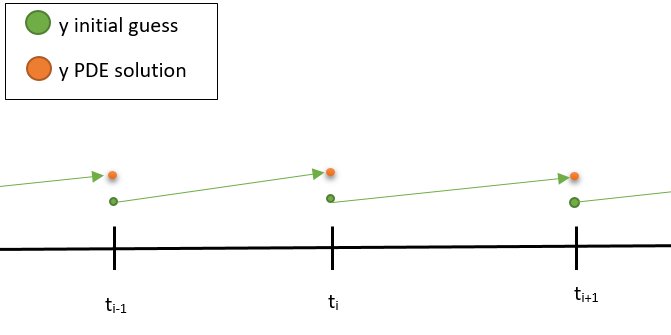
\includegraphics[width=9cm]{rhoSol.png}\\
		\caption{Multiple Shooting}
	\end{figure}	
\end{frame}


\begin{frame}
	\frametitle{Summary: What We Do}
 \begin{itemize}
 	\item Modelling multiscale particle dynamics.
 	\item Solving PDE-constrained optimization problems.
 	\item Using pseudospectral methods and multiple shooting for numerical solutions.
 	\item Application to industrial processes.
 \end{itemize}
	
\end{frame}

\begin{frame}
\frametitle{References}    
\begin{thebibliography}{10}    

	\bibitem{Jemand2000}
     T. Carraro, M. Geiger and R. Rannacher.
	\newblock {\em Indirect Multiple Shooting for Nonlinear Parabolic Optimal Control Problems with Control Constraints.}
	\newblock { \em SIAM Journal on Scientific Computing.} 36(2), 452-481, 2015.
	
	\bibitem{Jemand2000}
	J.C. De los Reyes.
	\newblock {\em Numerical PDE-Constrained Optimization.}
	\newblock 	Springer, 2015.
	
	\bibitem{Autor1990}
	A. Nold, B.D. Goddard, P. Yatsyshin, N. Savva and S. Kalliadasis. 
	\newblock {\em 	Pseudospectral Methods for Density Functional Theory in Bounded and 
		Unbounded Domains}.
	\newblock {\em Journal of Computational Physics}, 334, 639-664, 2017.
	\newblock \url{https://datashare.is.ed.ac.uk/handle/10283/2647} (2DChebClass)
	
\end{thebibliography}
\end{frame}


%By SunKart at English Wikipedia, CC BY 3.0, https://commons.wikimedia.org/w/index.php?curid=17582614 colloid picture
\end{document}